\def\assignmenttitle{Simulation of AR(p) and Seasonal processes}
\def\assignmentnumber{2}
\def\assignmentdate{11-10-2011}

\documentclass[11pt]{article}
\linespread{1}

\renewcommand{\thefootnote}{\fnsymbol{footnote}}

\usepackage{geometry} % see geometry.pdf on how to lay out the page. There's lots.
\usepackage[utf8]{inputenc}
\usepackage[T1]{fontenc}
\usepackage{array}
\usepackage{amsmath,amssymb,latexsym,epic,eepic,epsfig,graphics,psfrag}
\usepackage{amsfonts}
\usepackage{graphicx,float}
\usepackage{color}
\definecolor{mygray}{RGB}{244,244,244}
\definecolor{gray}{gray}{0.5}
\definecolor{myredish}{RGB}{193,33,97}
\definecolor{grayblue}{RGB}{91,112,142}
\definecolor{myorange}{RGB}{255,134,0}
\definecolor{green}{rgb}{0,0.4,0}

\usepackage[english]{babel}

\usepackage[bottom]{footmisc}

\usepackage{fancyhdr}
\pagestyle{fancy}
\lhead{\small\textit{Assignment \assignmentnumber -- 02417 Time Series Analysis -- Anders Hørsted (s082382)}}
\rhead{\thepage}
\chead{}
\lfoot{}\cfoot{}\rfoot{}

\usepackage{subfigure}
\usepackage{pstricks}
\usepackage{pst-node}
\usepackage{wrapfig}
\usepackage{caption}
\usepackage{multirow}
%\usepackage{fouriernc}
%\usepackage[charter]{mathdesign}
\usepackage{lmodern}
\usepackage[normalem]{ulem}
\geometry{a4paper} % or letter or a5paper or ... etc
% \geometry{landscape} % rotated page geometry

\usepackage{url}


\makeatletter
\renewcommand*\env@matrix[1][*\c@MaxMatrixCols c]{%
  \hskip -\arraycolsep
  \let\@ifnextchar\new@ifnextchar
  \array{#1}}
\makeatother

\newcommand\myimp{\quad\Leftrightarrow\quad}
\newcommand\half{\frac{1}{2}}
\newcommand\myvec[1]{\mathbf{#1}}
\newcommand\mymod[1]{\ (\text{mod }#1)}
\newcommand\myreal{\mathbb{R}}
\newcommand\mynatural{\mathbb{N}}
\newcommand\myinteger{\mathbb{Z}}
\newcommand\mycomplex{\mathbb{C}}
\newcommand\myint{\text{int}}
\newcommand\norm[1]{||\,#1\,||}
\newcommand\bignorm[1]{\big|\big|\,#1\,\big|\big|}
\newcommand\seq[1]{\big\{#1\big\}}
\newcommand\smallseq[1]{\{#1\}}
\newcommand\smallseqtoinf[1]{\smallseq{#1}_{k=1}^\infty}
\newcommand\lonew{\ell^1_w}
\newcommand\lone{\ell^1}
\newcommand\ltwo{\ell^2(\mynatural)}
\newcommand\ip[2]{\langle#1,#2\rangle}
\newcommand\hilbert[1]{\mathcal{#1}}
\newcommand\uinf{u_{\infty}}
\newcommand\erf{\text{erf\,}}
\newcommand\infint{\int_{\infty}^{\infty}}
\newcommand\fpi{FPI}
\newcommand\E[1]{\text{E}[#1]}
\newcommand\Var[1]{\text{Var}[#1]}
\newcommand\Cov[1]{\text{Cov}[#1]}
\newcommand\myverb[1]{{\footnotesize\texttt{#1}}}
\newcommand\Yhat{\widehat{Y}}
\newcommand\given{\,|\,}

\usepackage[scaled]{beramono}
\usepackage{listings}
\lstset {                 % A rudimentary config that shows off some features.
    language=R,
    basicstyle=\scriptsize\ttfamily, % Without beramono, we'd get cmtt, the teletype font.
    commentstyle=\textit, % cmtt doesn't do italics. It might do slanted text though.
    keywordstyle=,
    identifierstyle=,
    framextopmargin=4pt,
    framexbottommargin=4pt,
    framexleftmargin=4pt,
    framexrightmargin=4pt,
    xleftmargin=4pt,
    xrightmargin=4pt,
    backgroundcolor=\color{mygray},
    frame=single,
    showstringspaces=false,
    captionpos=b,
    tabsize=4            % Or whatever you use in your editor, I suppose.
}

\renewcommand{\lstlistlistingname}{Code Listings}
\renewcommand{\lstlistingname}{Code Listing}

\usepackage{tabulary}
\newcolumntype{y}{>{\centering\arraybackslash}R}

\title{\assignmenttitle}
\date{\assignmentdate}
\author{Assignment \assignmentnumber\ -- 02417 Time Series Analysis -- Anders Hørsted (s082382)}
%\author{}
\date{} % delete this line to display the current date



%%% BEGIN DOCUMENT
\begin{document}

\maketitle

This report consists of four parts. In the first part a few theoretical results for the AR(2) process are obtained and a prediction is made for a seasonal model. In part two a few different techniques for simulation of AR-processes are tested and the results from using different coefficients in the lag polynomial are compared and commented on. In part three the random walk process is simulated and plotted along with the autocorrelation function of the process. Finally in part four a couple of seasonal models are simulated and the autocorrelation function is plotted.

\section*{Part 1: Theory and prediction of seasonal model}
\subsection*{The AR(2)-process}
We consider the AR(2)-process
\begin{equation*}
    X_t + \phi_1 X_{t-1} + \phi_2 X_{t-2} = \varepsilon_t
\end{equation*}
where $\varepsilon_t$ is white noise. First the parameters for which the AR(2)-process is stationary are determined. \par

From theorem 5.9 in \cite{hm} the roots of the equation $\phi(z^{-1})=0$, with respect to $z$, should all lie within the unit circle for the AR(2)-process to be stationary. Now assuming $z\neq0$ we get
\begin{equation*}
    \phi(z^{-1}) = \phi_2 z^{-2} + \phi_1 z^{-1} + 1
\end{equation*}
so the roots are found from
\begin{align*}
    \phi_2 z^{-2} + \phi_1 z^{-1} + 1 &= 0 \myimp \\
    z^2 + \phi_1 z + \phi_2 &= 0
\end{align*}
With $D = \phi_1^2 - 4\phi_2$ we find the roots as
\begin{equation*}
    z_1 = \frac{-\phi_1 + \sqrt{D}}{2},\quad z_2 = \frac{-\phi_1 - \sqrt{D}}{2}
\end{equation*}
We now look at the three cases $D=0, D<0, D>0$ one at a time. \par

First $D=0$. Then we get a real double root given by $z_1=z_2=-\frac{\phi_1}{2}$ and since this root should be within the unit circle, we get the inequality
\begin{equation*}
    \frac{|\phi_1|}{2} < 1 \myimp \phi_1\in(-2, 2)
\end{equation*}
Since $D=0\Leftrightarrow\phi_1^2=4\phi_2$ we get the first set
\begin{equation*}
    M_1 = \{(\phi_1, \phi_2) \,|\, \phi_1^2=4\phi_2, \phi_1\in(-2,2)\}
\end{equation*}
for which the AR(2)-process is stationary \par
    For the second case $D<0$ we get two complex roots given by
\begin{equation*}
    z_1 = \frac{-\phi_1}{2} + \frac{\sqrt{4\phi_2 - \phi_1^2}}{2}\,i,\quad z_2\frac{-\phi_1}{2} - \frac{\sqrt{4\phi_2 - \phi_1^2}}{2}\,i
\end{equation*}
where both roots have the same modulus $|z_1|=|z_2|=\sqrt{\phi_2}$. Therefore to get stationarity $\sqrt{\phi_2}<1\Leftrightarrow\phi_2\in[0,1)$, which combined with $D<0 \Leftrightarrow \phi_1^2<4\phi_2$ gives $\phi_1\in(-2,2)$ and the second parameter set becomes
\begin{equation*}
    M2 = \{(\phi_1, \phi_2) \,|\, \phi_1^2<4\phi_2, \phi_1\in(-2,2)\}
\end{equation*}
For the last case $D>0$ the root of interest depends on the sign of $\phi_1$. If $\phi_1<0$ we look at $z_1$ and for $\phi_1>0$ we look at $z_2$. Both cases can be handled by one inequality given by
\begin{align*}
    \frac{|\phi_1| + \sqrt{\phi_1^2 - 4\phi_2}}{2} &< 1 \myimp\\
    |\phi_1| + \sqrt{\phi_1^2 - 4\phi_2} &< 2
\end{align*}
From this we get that $\phi_1\in(-2,2)$. We now look at all lines for which $\phi_2=|\phi_1|-1$, giving
\begin{align*}
    |\phi_1| + \sqrt{\phi_1^2 - 4\phi_2} &= |\phi_1| + \sqrt{\phi_1^2 - 4(|\phi_1|-1)} \\
    &= |\phi_1| + \sqrt{(|\phi_1|-2)^2} \\
    &= |\phi_1| + |\,|\phi_1|-2\,| \\
    &= 2
\end{align*}
using that for $\phi_1\in(-2,2),\:|\,|\phi_1|-2\,|=2-|\phi_1|$. From the expression for $D$ we conclude that $\phi_2>|\phi_1|-1$. Combined with $D>0\Leftrightarrow \frac{1}{4}\phi_1^2>\phi_2$ the last set is
\begin{equation*}
    M_3 = \{(\phi_1, \phi_2) \,|\, |\phi_1|-1<\phi_2<\frac{1}{4}\phi_1^2, \phi_1\in(-2,2)\}
\end{equation*}
The final result is that the AR(2)-process is stationary for parameters in the set
\begin{equation*}
    M = M_1 \cup M_2 \cup M_3 = \{(\phi_1, \phi_2) \,|\, |\phi_1| - 1 < \phi_2 < 1\}
\end{equation*}
The set $M$ is sketched in figure~\ref{fig:part1-stationary}. \par

\begin{figure}
    \centering
    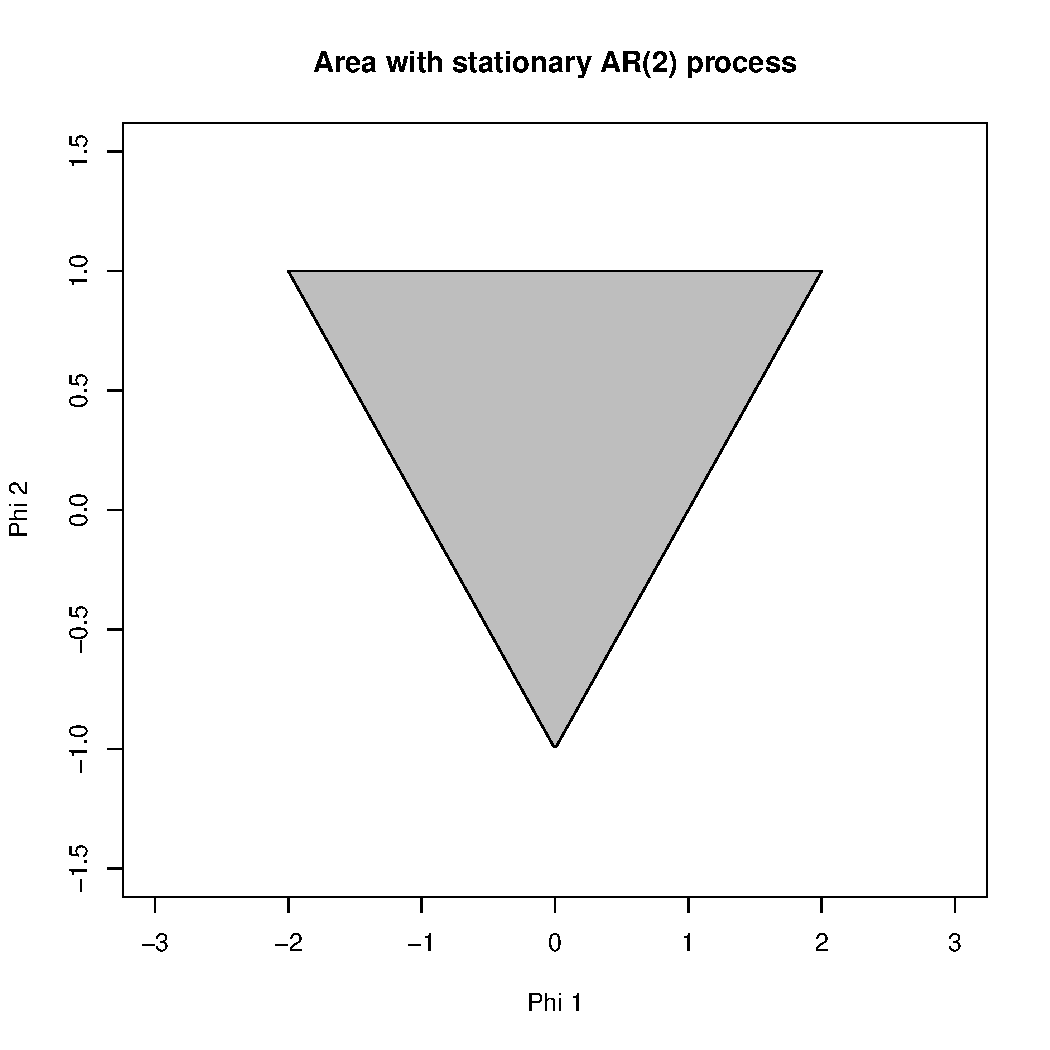
\includegraphics[width=80mm]{part1-stationary.pdf}
    \caption{\textit{Set of the $(\phi_1, \phi_2)$-plane where the characteristic equation for an AR(2) process has roots within the unit circle.}}
    \label{fig:part1-stationary}
\end{figure}

We now need to determined the set of parameters for which the autocorrelation function of the AR(2)-process shows damping harmonic oscillations. Based on equation 5.83 and the surrounding text in \cite{hm} the autocorrelation function shows damping harmonic oscillations exactly when the roots of the characteristic equation are complex. Using the result from the previous paragraphs the set where the autocorrelation function shows damping harmonic oscillations is given by
\begin{equation*}
    M2 = \{(\phi_1, \phi_2) \,|\, \phi_1^2<4\phi_2, \phi_1\in(-2,2)\}
\end{equation*}
The set $M2$ is sketched in figure~\ref{fig:part1-damping}

\begin{figure}
    \centering
    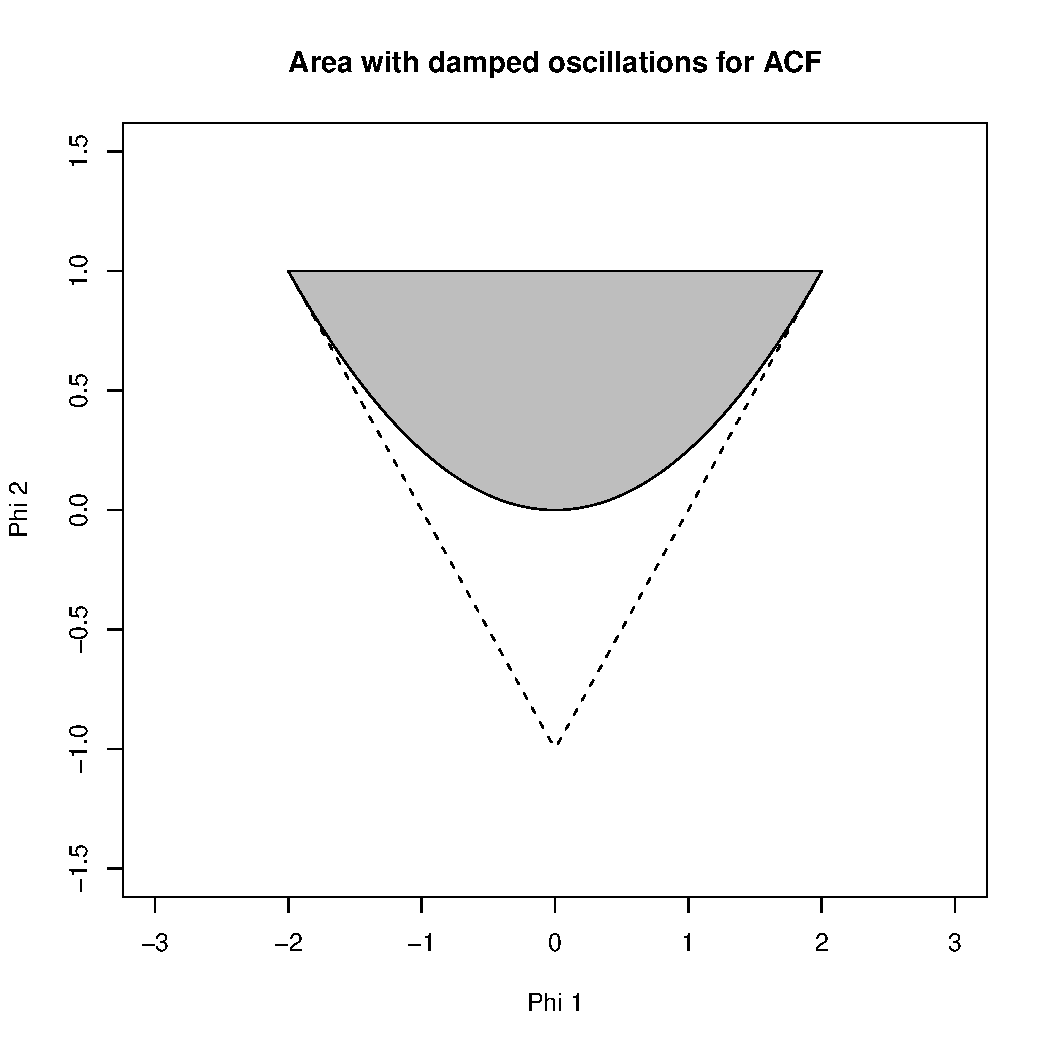
\includegraphics[width=80mm]{part1-damping.pdf}
    \caption{\textit{Set of the $(\phi_1, \phi_2)$-plane where the autocorrelation function for an AR(2) process shows damping harmonic oscillations.}}
    \label{fig:part1-damping}
\end{figure}

\subsection*{Prediction in seasonal model}
We now model the deviation $Y_t$ between observed and calculated water levels as a linear model given by
\begin{equation}\label{eq:predict}
    (1-0.8B)(1-0.2B^6)(1-B)Y_t = \varepsilon_t
\end{equation}
where $\varepsilon_t$ is white noise with variance $\sigma^2_\varepsilon$. An estimate based on around 1500 observations is calculated as $\hat{\sigma}^2_\varepsilon=0.31\,\text{dm}^2$. Based on the data $D=\{Y_1, Y_2, \dots, Y_{10}\}$ shown in table 1 in the assignment paper, we will predict $Y_{12}$.\par
First the operator polynomial in model (\ref{eq:predict}) is expanded giving
\begin{align*}
    (1 - 1.8B + 0.8B^2 - 0.2B^6 + 0.36B^7 - 0.16B^8)Y_t = \varepsilon_t 
\end{align*}
that rewritten gives 
\begin{equation*}
    Y_t = 1.8Y_{t-1} - 0.8Y_{t-2} + 0.2Y_{t-6} - 0.36Y_{t-7} + 0.16Y_{t-8} + \varepsilon_t
\end{equation*}
We can now predict $Y_t$ at time $t=11$ by
\begin{align*}
    \widehat{Y}_{11} &= \E{Y_{11}\given D}\\
    &= 1.8Y_{10} - 0.8Y_9 + 0.2Y_5 -0.36Y_4 + 0.16Y_3\\
    &= -5.44
\end{align*}
The prediction $\Yhat_{11}$ is then used to find $\Yhat_{12}$
\begin{align*}
    \Yhat_{12} &= \E{Y_{12}\given D} \\
    &= 1.8\Yhat_{11} - 0.8Y_{10} + 0.2Y_6 - 0.36Y_5 + 0.16Y_4 \\
    &= -6.43
\end{align*}
To get a 95\% confidence interval for $\Yhat_{12}$ we need to find the variance of the prediction error $Y_{12}-\Yhat_{12}$.
\begin{align*}
    \Var{Y_{12} - \Yhat_{12}\given D} &= \Var{1.8Y_{11} + \varepsilon_{12}\given D} \\
    &= \Var{1.8(1.8Y_{10} - 0.8Y_9 + 0.2Y_5 -0.36Y_4 + 0.16Y_3 + \varepsilon_{11}) + \varepsilon_{12}\given D} \\
    &= \Var{1.8\varepsilon_{11} + \varepsilon_{12}} \\
    &= (1.8^2 + 1)\sigma^2_\varepsilon
\end{align*}
Since $\sigma^2_\varepsilon$ is unknown we use the estimate $\hat{\sigma}^2_\varepsilon$ instead which gives
\begin{align*}
    \Var{Y_{12} - \Yhat_{12}\given D} &= (1.8^2 + 1)\hat{\sigma}^2_\varepsilon \\
    &= 1.31
\end{align*}
And finally we get the 95\% confidence interval for $\Yhat_{12}$ as
\begin{equation*}
    -6.43\pm 1.96\cdot\sqrt{1.31} = [-8.68; -4.18]
\end{equation*}

\section*{Part 2: Simulating AR-processes}
In this part we will simulate a few different AR-processes using the \myverb{filter} and \myverb{arima.sim} functions in R. The AR(2)-process is written as 
\begin{equation*}
    Y_t = a_1Y_{t-1} + a_2Y_{t-2} + e_t
\end{equation*}

\subsection*{Simulating the AR(1)-process}
We first simulate the AR(1)-process for coefficients $a_1=0.1, -0.1, 0.9, -0.9$ and $a_2=0$. The results are shown in figure~\ref{fig:ar1-filter-1} and figure~\ref{fig:ar1-filter-2}. From the figures it is seen that the ACF for the two models with numerically small $a_1$ decays rapidly to zero while the ACF for the models with numerically large $a_1$ decays slower. The model with numerically small $a_1$ is looking much like white noise, while the models with numerically large coefficients seems closer to a non-stationary process. The extreeme case where $|a_1|>1$ is plotted in figure~\ref{fig:ar1-filter-3} and it is seen that the ACFs for these functions are almost constant which shows that these processes are indeed non-stationary. This corresponds with the fact that the root of the characteristic equation for an AR(1)-process is equal to $-a_1$, so for $|a_1|>1$ the absolute value of the root will also be greater than one. From theorem 5.9 in \cite{hm} we get that the AR process is non-stationary for roots with abolute value greater than one which match the results in the plots.

\begin{figure}
    \centering
    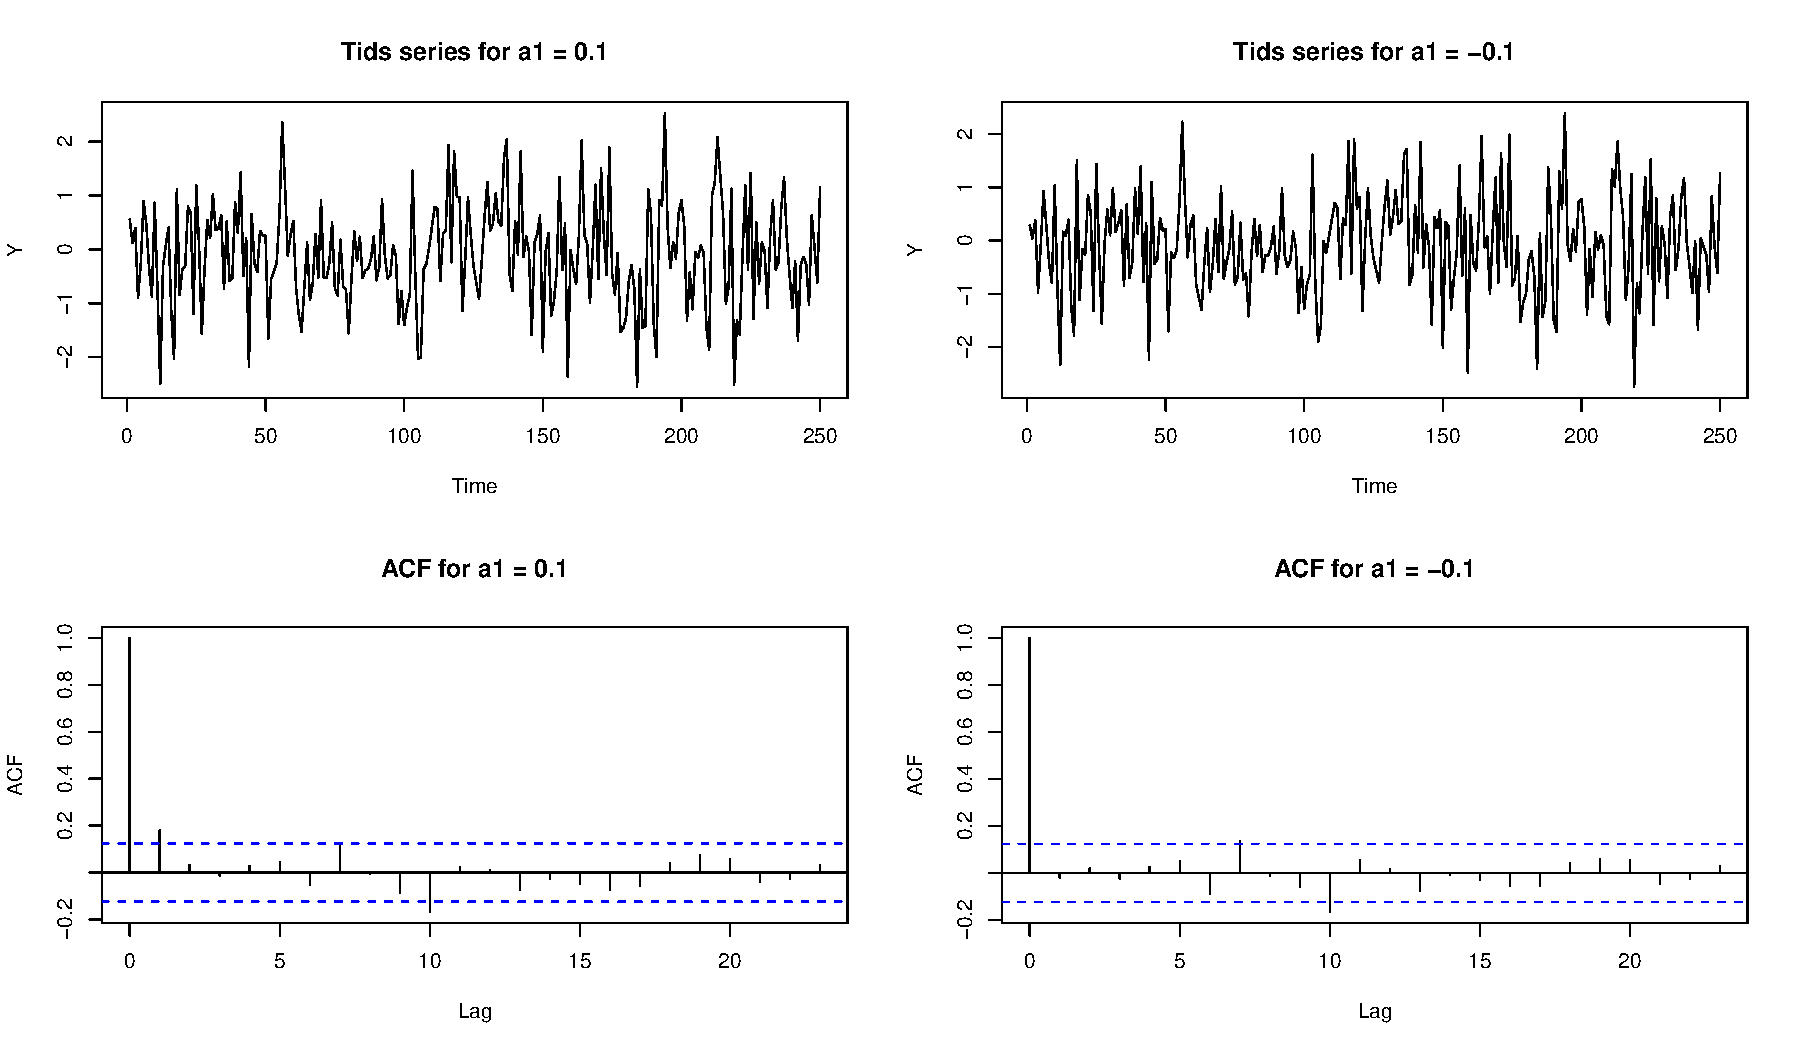
\includegraphics[width=140mm]{ar1-filter-1.pdf}
    \caption{\textit{Simulation of the AR(1)-process (with $a_1=0.1$ and $a_1=-0.1$) using the \myverb{filter} function}}
    \label{fig:ar1-filter-1}
\end{figure}

\begin{figure}
    \centering
    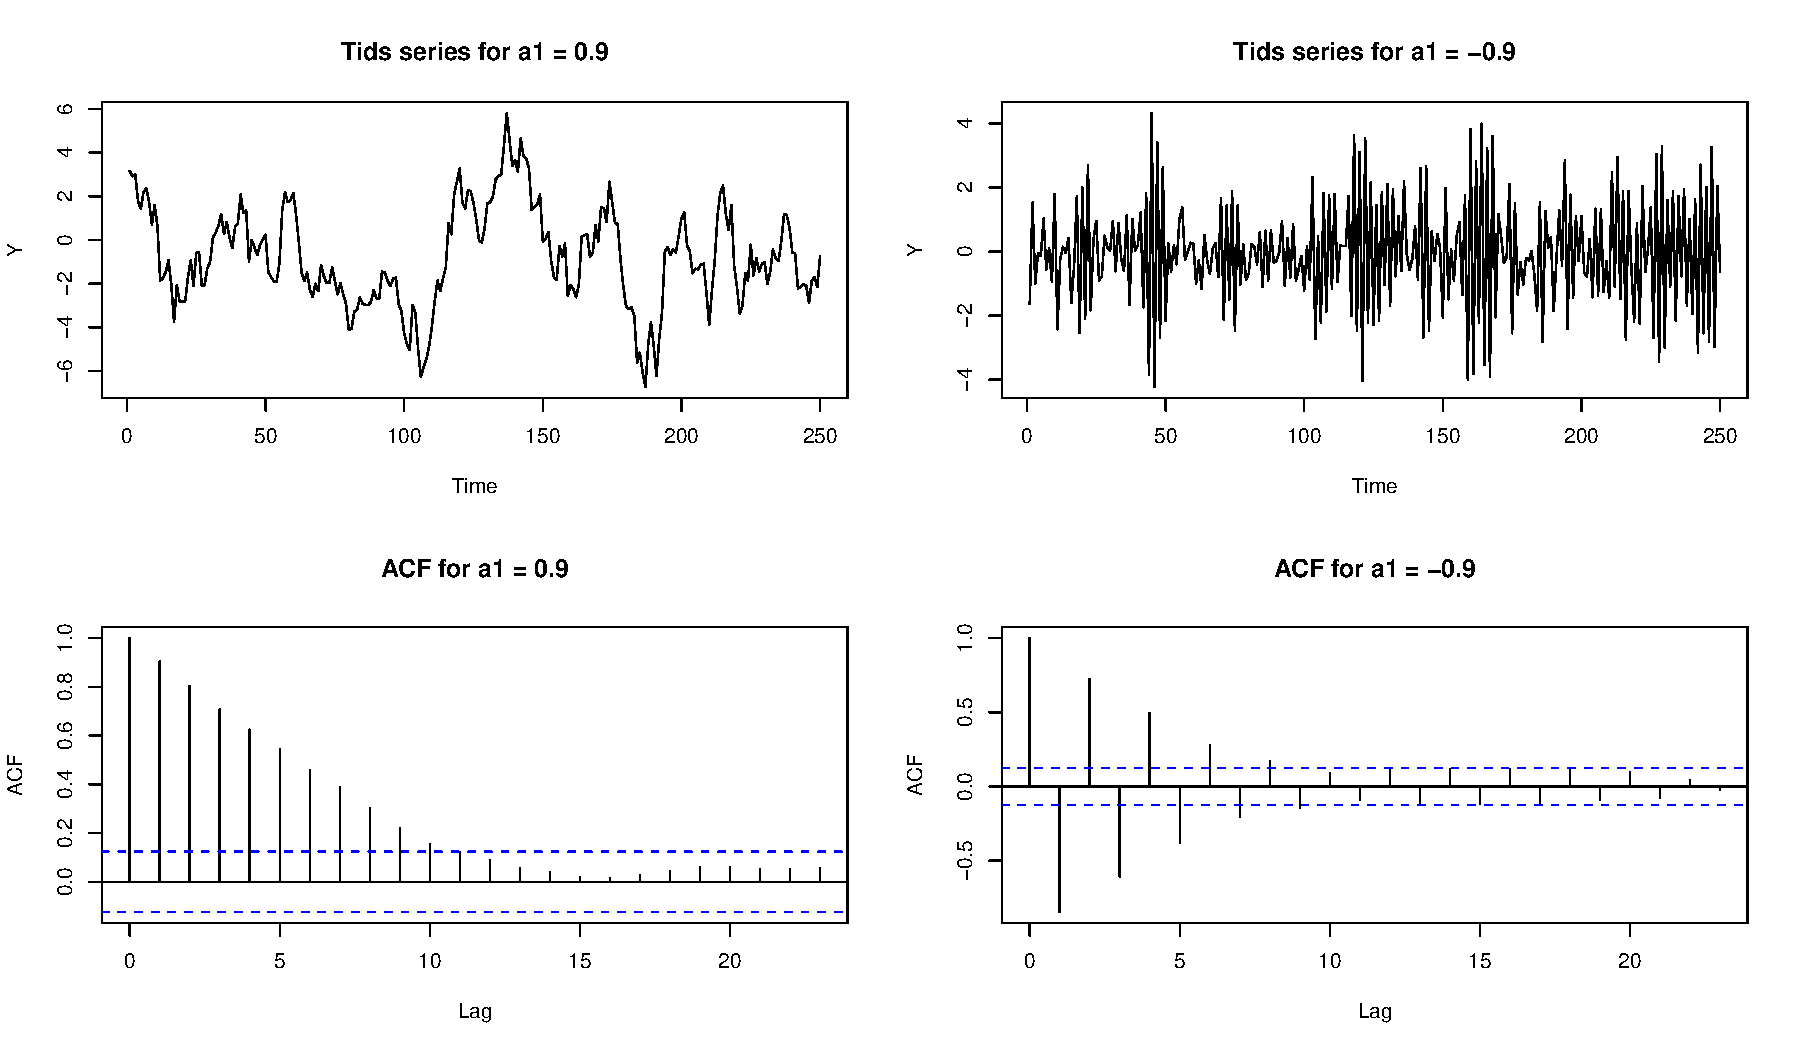
\includegraphics[width=140mm]{ar1-filter-2.pdf}
    \caption{\textit{Simulation of the AR(1)-process (with $a_1=0.9$ and $a_1=-0.9$) using the \myverb{filter} function}}
    \label{fig:ar1-filter-2}
\end{figure}

\begin{figure}
    \centering
    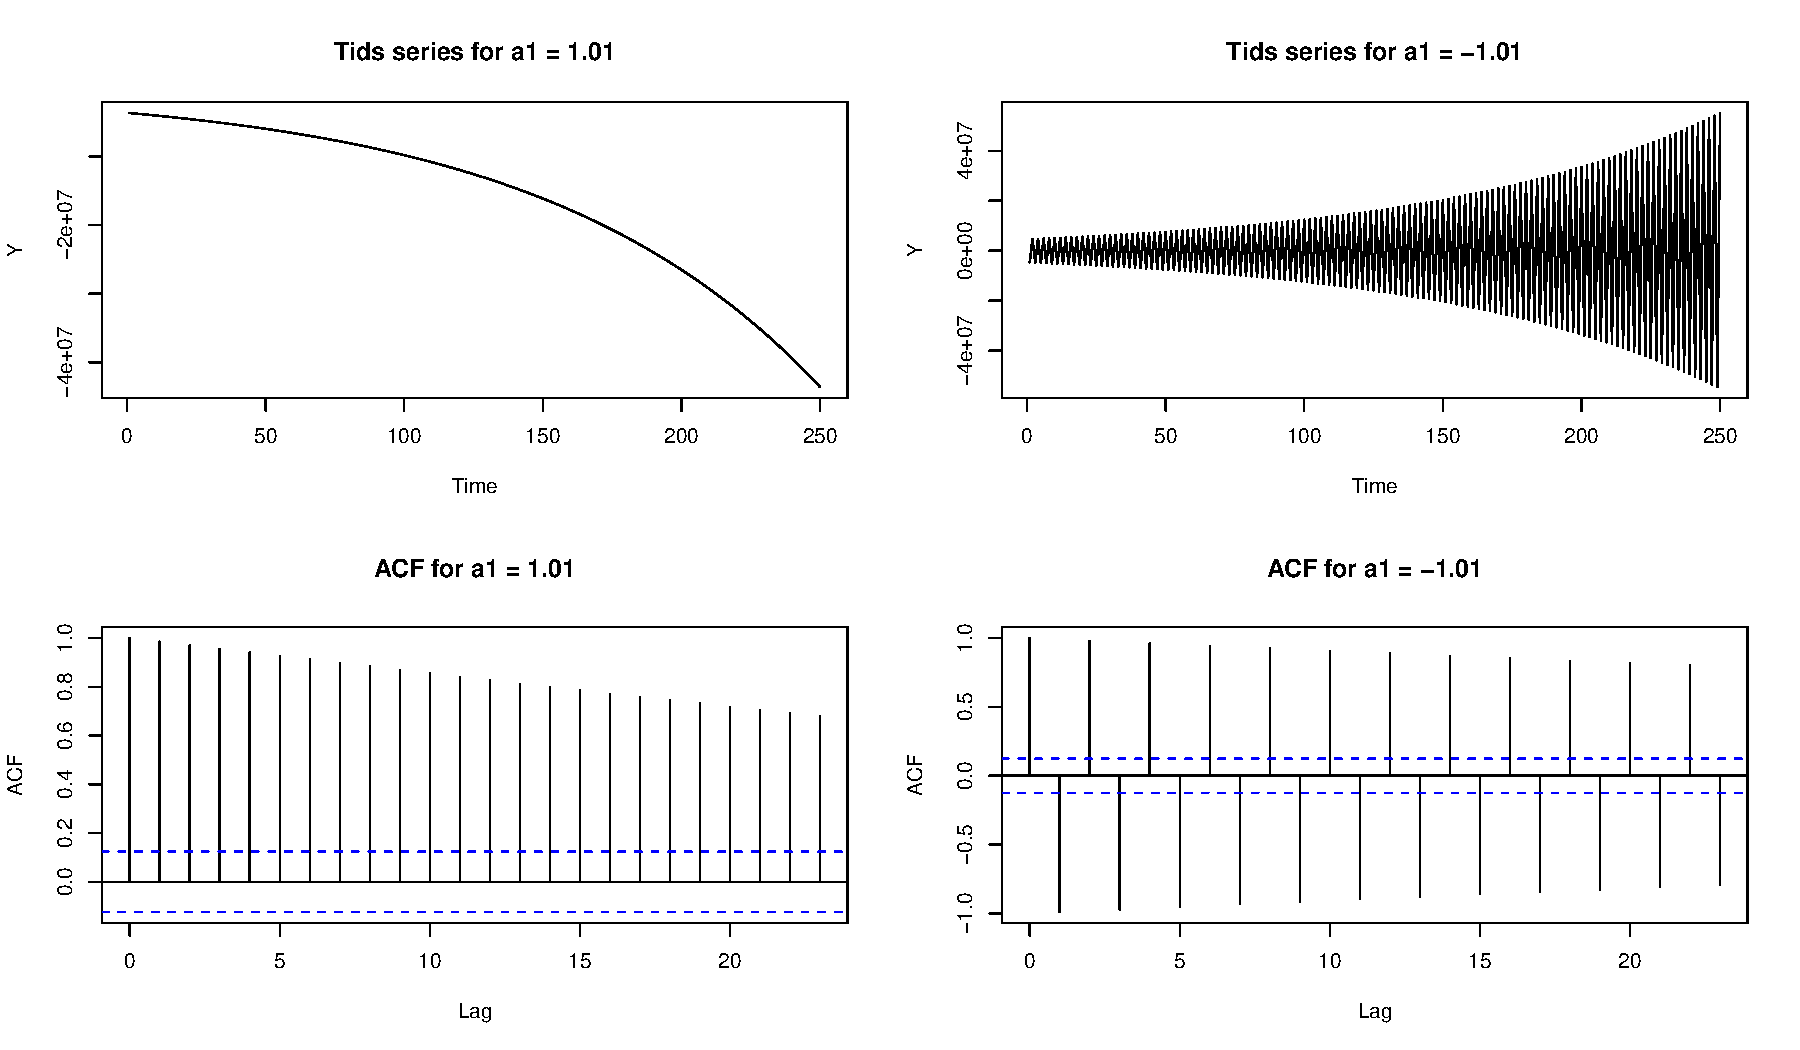
\includegraphics[width=140mm]{ar1-filter-3.pdf}
    \caption{\textit{Simulation of the AR(1)-process (with $a_1=1.01$ and $a_1=-1.01$) using the \myverb{filter} function}}
    \label{fig:ar1-filter-3}
\end{figure}

\subsection*{Simulating the AR(2)-process}
Next we will simulate an AR(2)-process. To make sure the process is stationary we choose two roots $-1<r_1, r_2<1$ and then calculate
\begin{align*}
    (x-r_1)(x-r_2) &= x^2 - (r_1+r_2)x + r_1r_2
\end{align*}
from which we see that we should choose $a_1=r_1+r_2$ and $a_2=-r_1r_2$. Two pairs of roots are now selected as $(-\frac{1}{2}, \frac{3}{4}), (\frac{2}{5}, \frac{9}{10})$ and the AR(2)-process is simulated, using the \myverb{filter} function, for these two models. The results are shown in figure~\ref{fig:ar2-filter-1}. In the figure it seen that the ACF decays relatively fast for both models, which was expected since both models are staionary. The same models are simulated with the \myverb{arima.sim} function and the results are shown in figure~\ref{fig:ar2-sim-1}. The same damping behaviour of the ACFs are observed although the ACF of the right model have values above the 95\%-prediction interval for lags around 20-25. It could look like a damped sine function, which still corresponds nicely with a non-stationary function. 

\begin{figure}
    \centering
    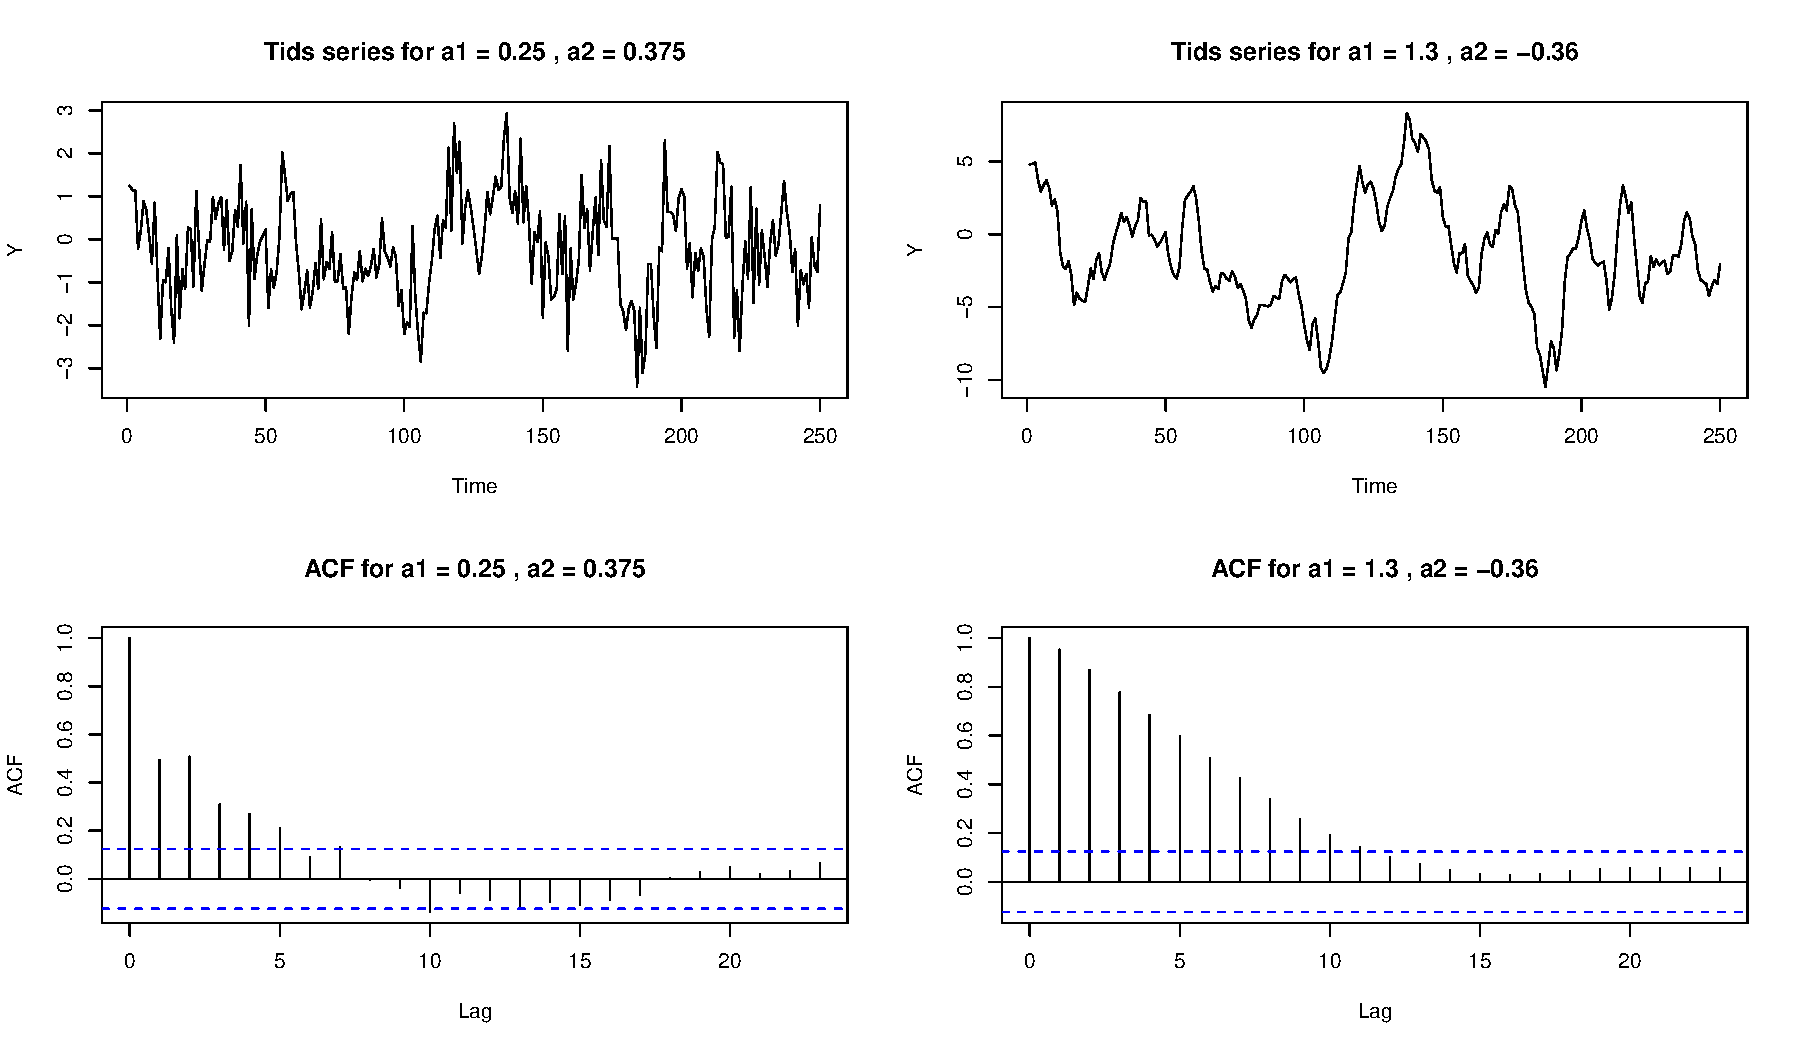
\includegraphics[width=140mm]{ar2-filter-1.pdf}
    \caption{\textit{Simulation of AR(2)-process using the \myverb{filter} function}}
    \label{fig:ar2-filter-1}
\end{figure}

\begin{figure}
    \centering
    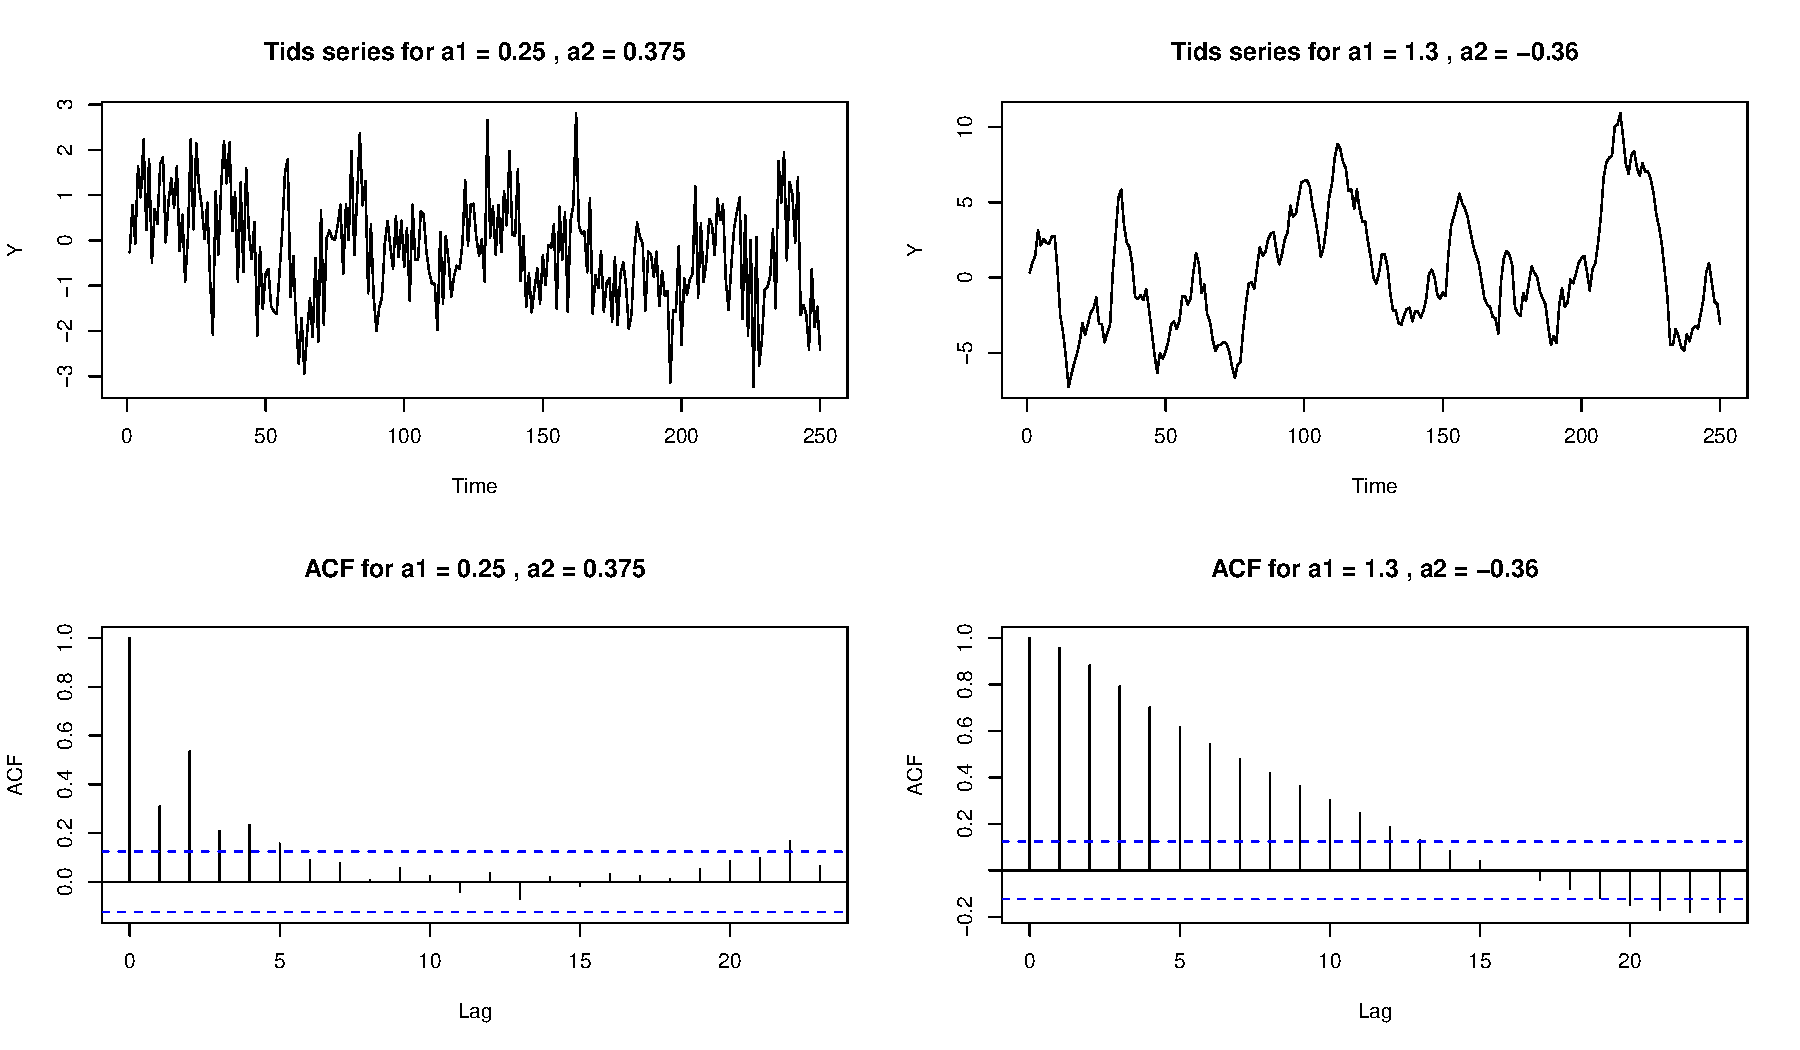
\includegraphics[width=140mm]{ar2-sim-1.pdf}
    \caption{\textit{Simulation of AR(2)-process using the \myverb{arima.sim} function}}
    \label{fig:ar2-sim-1}
\end{figure}

\section*{Part 3: Random Walk}
We start out by looking at the process given by
\begin{equation}\label{eq:random}
    Y_t = \sum_{s=0}^t e_s
\end{equation}
where $e_s$ is white noise with variance $\sigma^2_e$. Then the expectation of the process is
\begin{align*}
    \E{Y_t} &= \sum_{s=0}^t\E{e_s}\\
    &= 0
\end{align*}
Since the different $e_s$ are uncorrelated the covariance function can be found as
\begin{align*}
    \gamma(t, u) &= \Cov{Y_t, Y_u} \\
    &= \Cov{\sum_{s=0}^t e_s, \sum_{s=0}^u e_s} \\
    &= \sum_{s=0}^{\text{min}(t, u)} \Cov{e_s, e_s} \\
    &= (\text{min}(t,u) + 1)\cdot\sigma^2_e
\end{align*}
and then the variance is given by
\begin{align*}
    \Var{Y_t} &= \gamma(t,t) \\
    &= (t+1)\sigma^2_e
\end{align*}
Since the covariance depends on the time $t$ we get from definition 5.3 in \cite{hm} that the process (\ref{eq:random}) isn't stationary. To get a better view of the process we now simulate and plot the process. The process can easily be simulated by using the built-in \myverb{cumsum} function in R
\lstinputlisting[firstline=1,lastline=3]{part3.R}
Using this function we now simulate the process and plot it along with the estimated autocorrelation function. The plot is seen in figure~\ref{fig:randomwalk} and it is seen that the ACF is almost constant 1 for lags up to 35. This corresponds with the previous paragraph where the process was found to be non-stationary. To further illustrate the point, 6 simulations of the random walk are plotted in figure~\ref{fig:multiple-randomwalks}. From the figure it is seen that all 6 processes show some kind of trend, which further illustrates the non-stationarity of the random walk process. \par
We can now try to remove the non-stationarity by defining a new process as
\begin{equation*}
    X_t = Y_t - Y_{t-1}
\end{equation*}
and then plot this process along with its estimated auto correlation function. The plot is shown in figure~\ref{fig:randomwalkdiffed} and it is seen that the new process resembles white noise. This isn't surprising since
\begin{align*}
    Y_t - Y_{t-1} &= \sum_{s=0}^t e_s - \sum_{s=0}^{t-1} e_s \\
    &= e_t
\end{align*}
which shows that the process $\{X_t\}$ is in fact white noise.


\begin{figure}
    \centering
    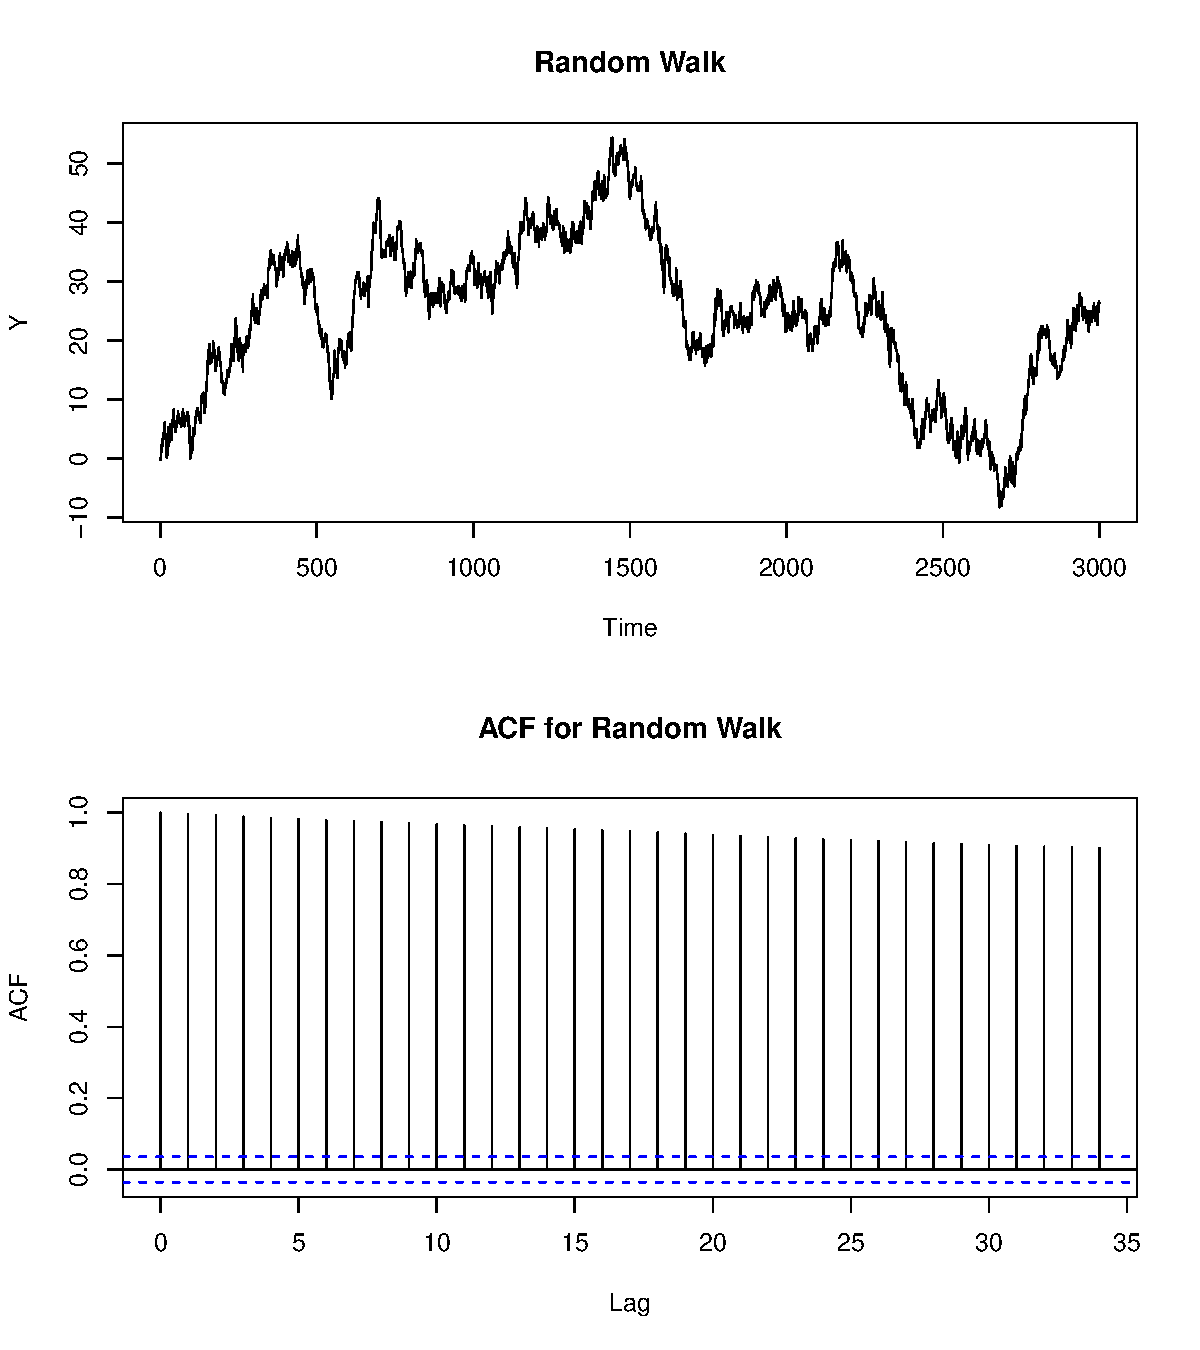
\includegraphics[width=80mm]{random-walk.pdf}
    \caption{\textit{Simulation of the Random Walk process using the \myverb{rnorm} and \myverb{cumsum} function in R}}
    \label{fig:randomwalk}
\end{figure}

\begin{figure}
    \centering
    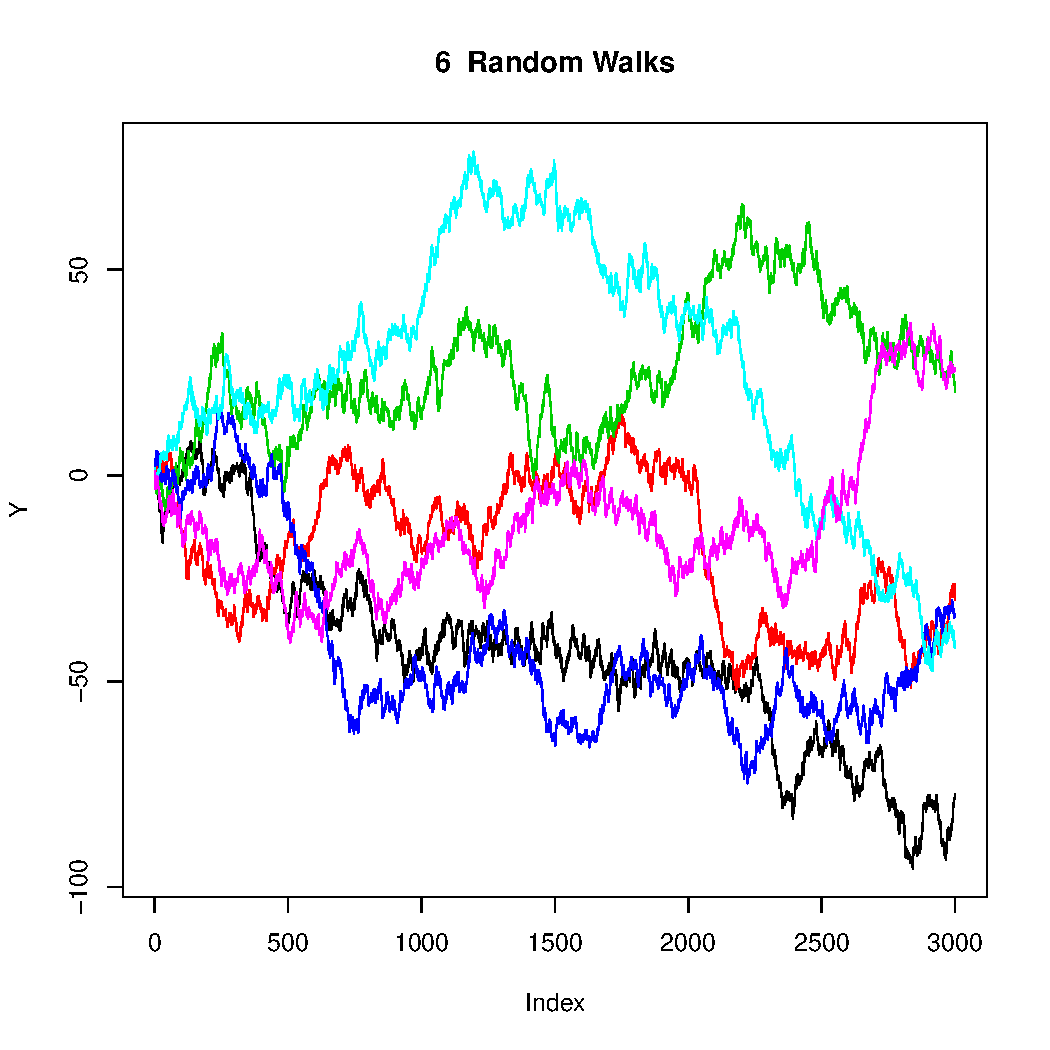
\includegraphics[width=80mm]{multiple-random-walk.pdf}
    \caption{\textit{Simulation of 6 Random Walk processes}}
    \label{fig:multiple-randomwalks}
\end{figure}

\begin{figure}
    \centering
    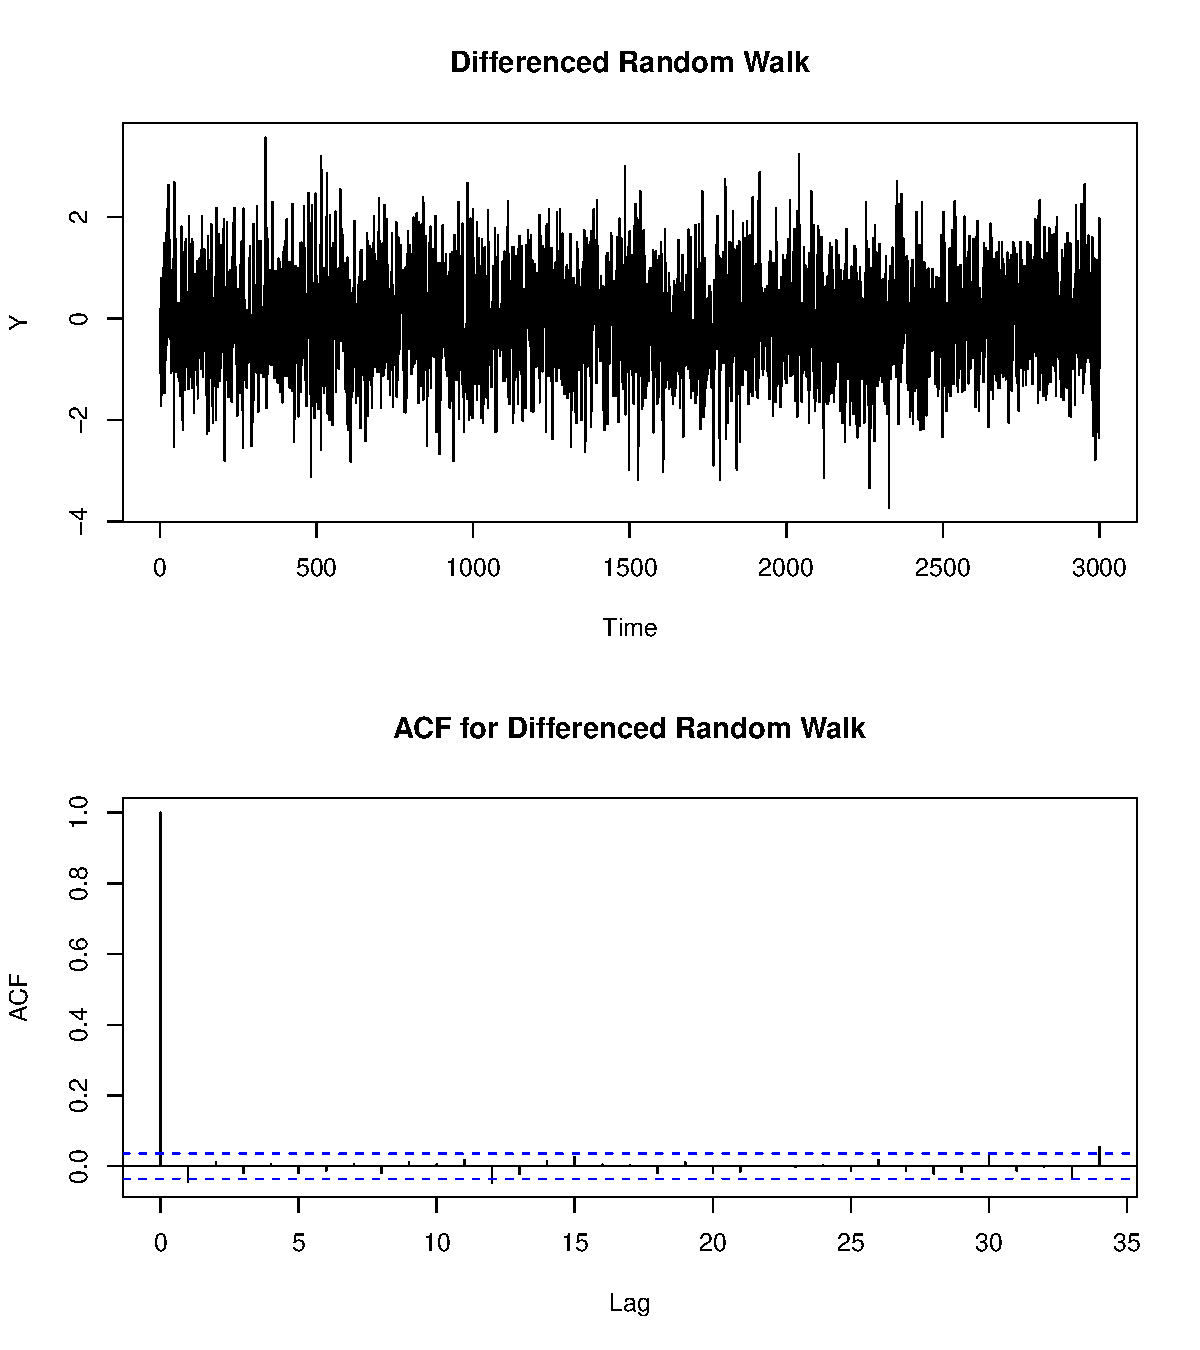
\includegraphics[width=80mm]{random-walk-diffed.pdf}
    \caption{\textit{Simulation of the process constructed by taking first differences of the Random Walk process}}
    \label{fig:randomwalkdiffed}
\end{figure}

\section*{Part 4: Seasonal processes}
In this section we will simulate multiplicative $(p,d,q)\times(P,D,Q)_s$ seasonal models on the form
\begin{equation*}
    \varphi(B)\phi(B^s)\nabla^d\nabla^D_sY_t = \theta(B)\Theta(B^s)\varepsilon_t
\end{equation*}
Since the \myverb{arima.sim} function can only simulate non-seasonal models, we have to expand the operator polynomials for some of the models before simulating them in R. The 6 models we are going to simulate are
\begin{itemize}
    \item \textbf{The $(1,0,0)\times(0,0,0)_{12}$ model} with $\varphi_1=0.9$\\
        This is just a regular AR(1) process so no expansion is needed
    \item \textbf{The $(0,0,0)\times(1,0,0)_{12}$ model} with $\phi_1=0.7$\\
        This is a seasonal AR(1) process but can also be seen as an AR(12) process, so no expansion is needed
    \item \textbf{The $(1,0,0)\times(0,0,1)_{12}$ model} with $\varphi_1=0.9, \Theta_1=0.4$\\
        This can be regarded as an ARMA(1,12) process and no expansion is needed
    \item \textbf{The $(1,0,0)\times(1,0,0)_{12}$ model} with $\varphi_1=0.9, \phi_1=0.7$\\
        This model needs to be expanded to give
        \begin{align*}
            (1 + \varphi_1 B)(1 + \phi_1 B^{12})Y_t &= \varepsilon_t \myimp\\
            (1 + \varphi_1 B + \phi_1 B^{12} + \varphi_1\phi_1 B^{13})Y_t &= \varepsilon_t
        \end{align*}
        which is an AR(13) process
    \item \textbf{The $(0,0,1)\times(0,0,1)$ model} with $\theta_1=0.4, \Theta_1=0.3$\\
        This model should also be expanded to give
        \begin{align*}
            Y_t &= (1 + \theta_1 B)(1 + \Theta_1 B^{12})\varepsilon_t \myimp\\
            Y_t &= (1 + \theta_1 B + \Theta_1 B^{12} + \theta_1\Theta_1 B^{13})\varepsilon_t
        \end{align*}
        which is an MA(13) process
    \item \textbf{The $(0,0,1)\times(1,0,0)_{12}$ model} with $\theta_1=0.4, \phi_1=0.7$\\
        This model can be seen as an ARMA(12,1) process and needs no expansion
\end{itemize}
With the expansions above, the 6 models are now simulated and the results are plotted in figure~\ref{fig:p4-1} and figure~\ref{fig:p4-2}. From the figures a few things are worth noticing. 
\begin{itemize}
    \item \textbf{The $(1,0,0)\times(0,0,0)_{12}$ model} with $\varphi_1=0.9$ is just an AR(1)-process and therefore the ACF decays. But the decay is slow corresponding to a root with absolute value close to 1. This is the same result as was found in part 2.
    \item \textbf{For the $(0,0,0)\times(1,0,0)_{12}$ model} with $\phi_1=0.7$ we see a high value of the ACF for lag 12, which we would expect since the seasonal length is 12. The characteristic equation for the model have 12 complex roots $r$ with $|r|=0.971$ for all roots. The process is stationary and what is seen in the ACF could be a slow decaying sine function.
    \item \textbf{The $(1,0,0)\times(0,0,1)_{12}$ model} with $\varphi_1=0.9, \Theta_1=0.4$ is an ARMA(1,12) and as mentioned on page 127 in \cite{hm} the ACF consists of damped exponential and harmonic functions only from lag $k=q+1-p$, which in this case is lag 12. This may explain the slow decay for this stationary process. 
    \item \textbf{The $(1,0,0)\times(1,0,0)_{12}$ model} with $\varphi_1=0.9, \phi_1=0.7$ is an AR(13) process and by solving
        \begin{equation*}
            z^{13} + 0.9z^{12} + 0.7z + 0.63 = 0
        \end{equation*}
        it is found that the characteristic equation has one negative real root and 6 pairs of complex conjugated roots. By the comments on page 122 in \cite{hm} we would expect a combination a shifting positive and negative exponentially decreasing function and damped waves. This is excatly what is seen in the plot.
    \item \textbf{The $(0,0,1)\times(0,0,1)$ model} with $\theta_1=0.4, \Theta_1=0.3$ is a MA(13) process and from table 6.1 in \cite{hm} we should expect the ACF to be 0 for lags greater than 13. Except from lag 15 this seems to be the case.
    \item \textbf{The $(0,0,1)\times(1,0,0)_{12}$ model} with $\theta_1=0.4, \phi_1=0.7$ is an ARMA(12,1) process and from page 126 in \cite{hm} we should expect that it consists of damped exponential and sine functions. In this case it seems to consist of sine functions.
\end{itemize}
To conclude it is seen that the ACF for lag 12 is high in model 2, 5 and 6. Model 1 isn't a seasonal model so it is natural that the ACF isn't high in this model at lag 12. A slightly higher correlation at lag 12 is also seen in model 4, although it isn't significant. Also the rate of decay in model 3 seems to slow down at lag 12, but this is also not significant.

\begin{figure}
    \centering
    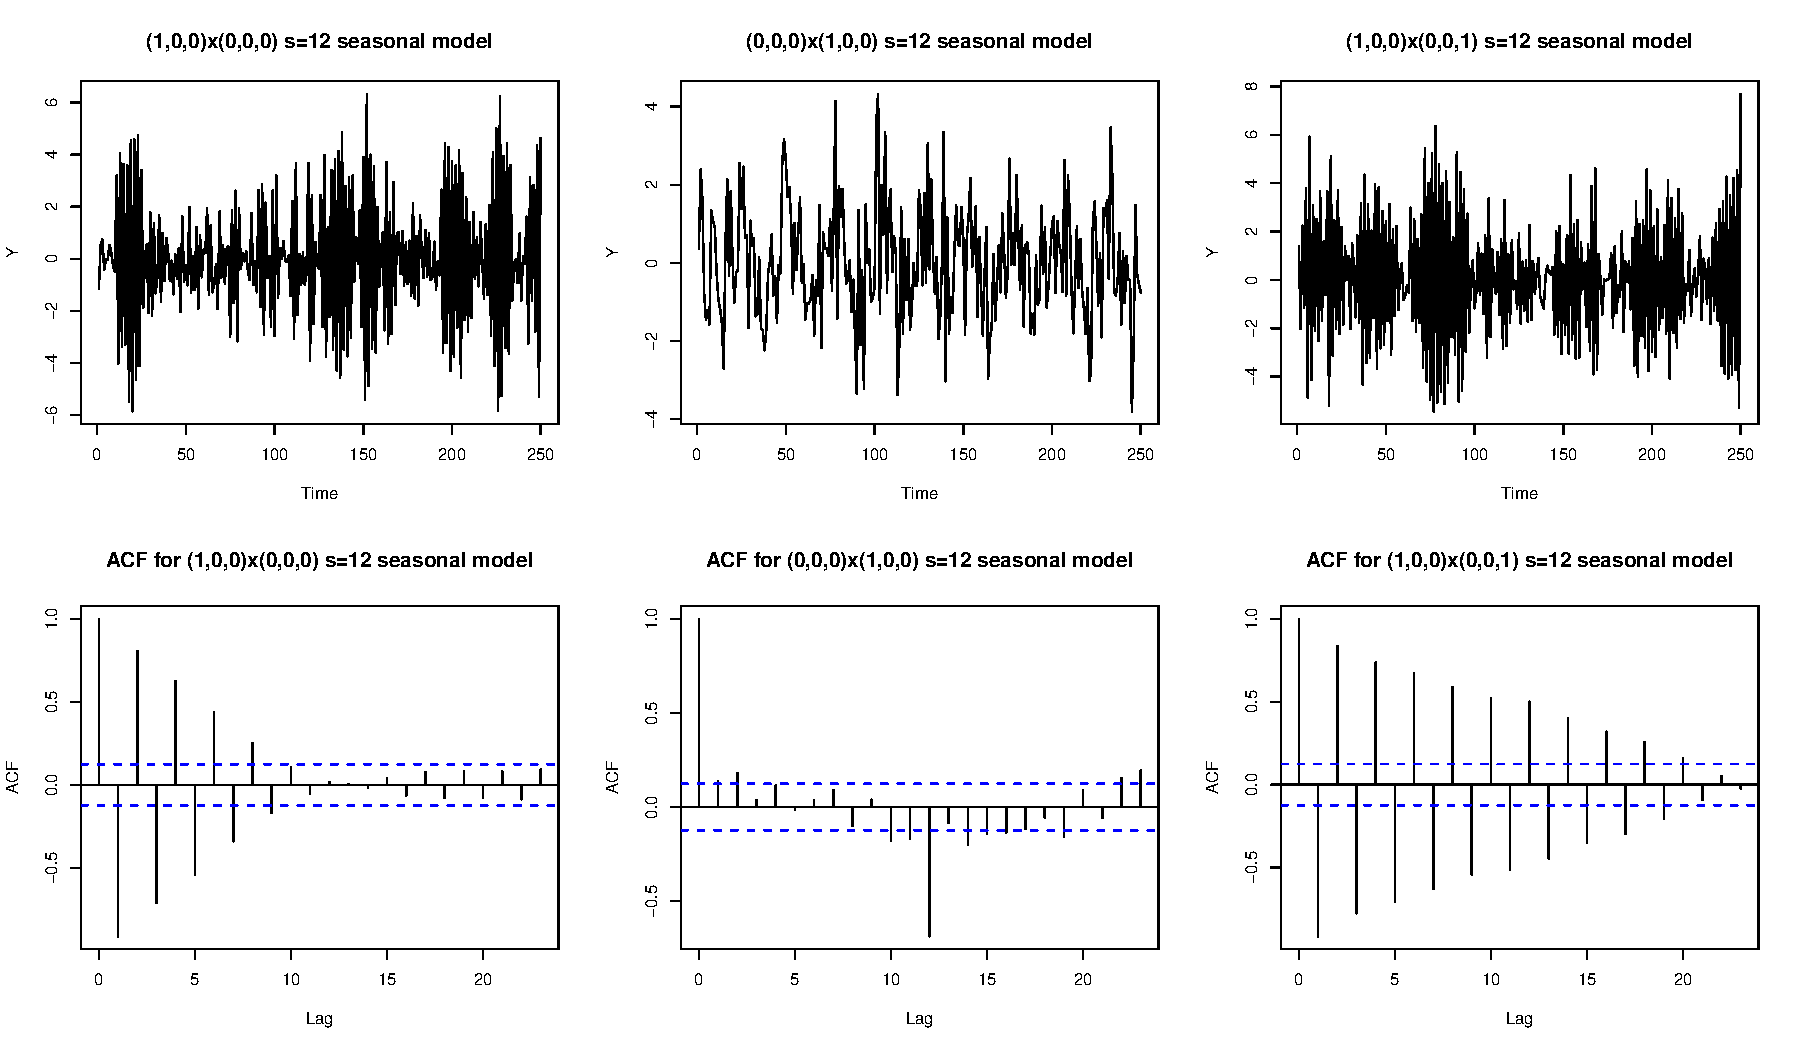
\includegraphics[width=140mm]{seasonalmodels-1.pdf}
    \caption{\textit{Simulation of the first 3 seasonal models in part 4.}}
    \label{fig:p4-1}
\end{figure}
\begin{figure}
    \centering
    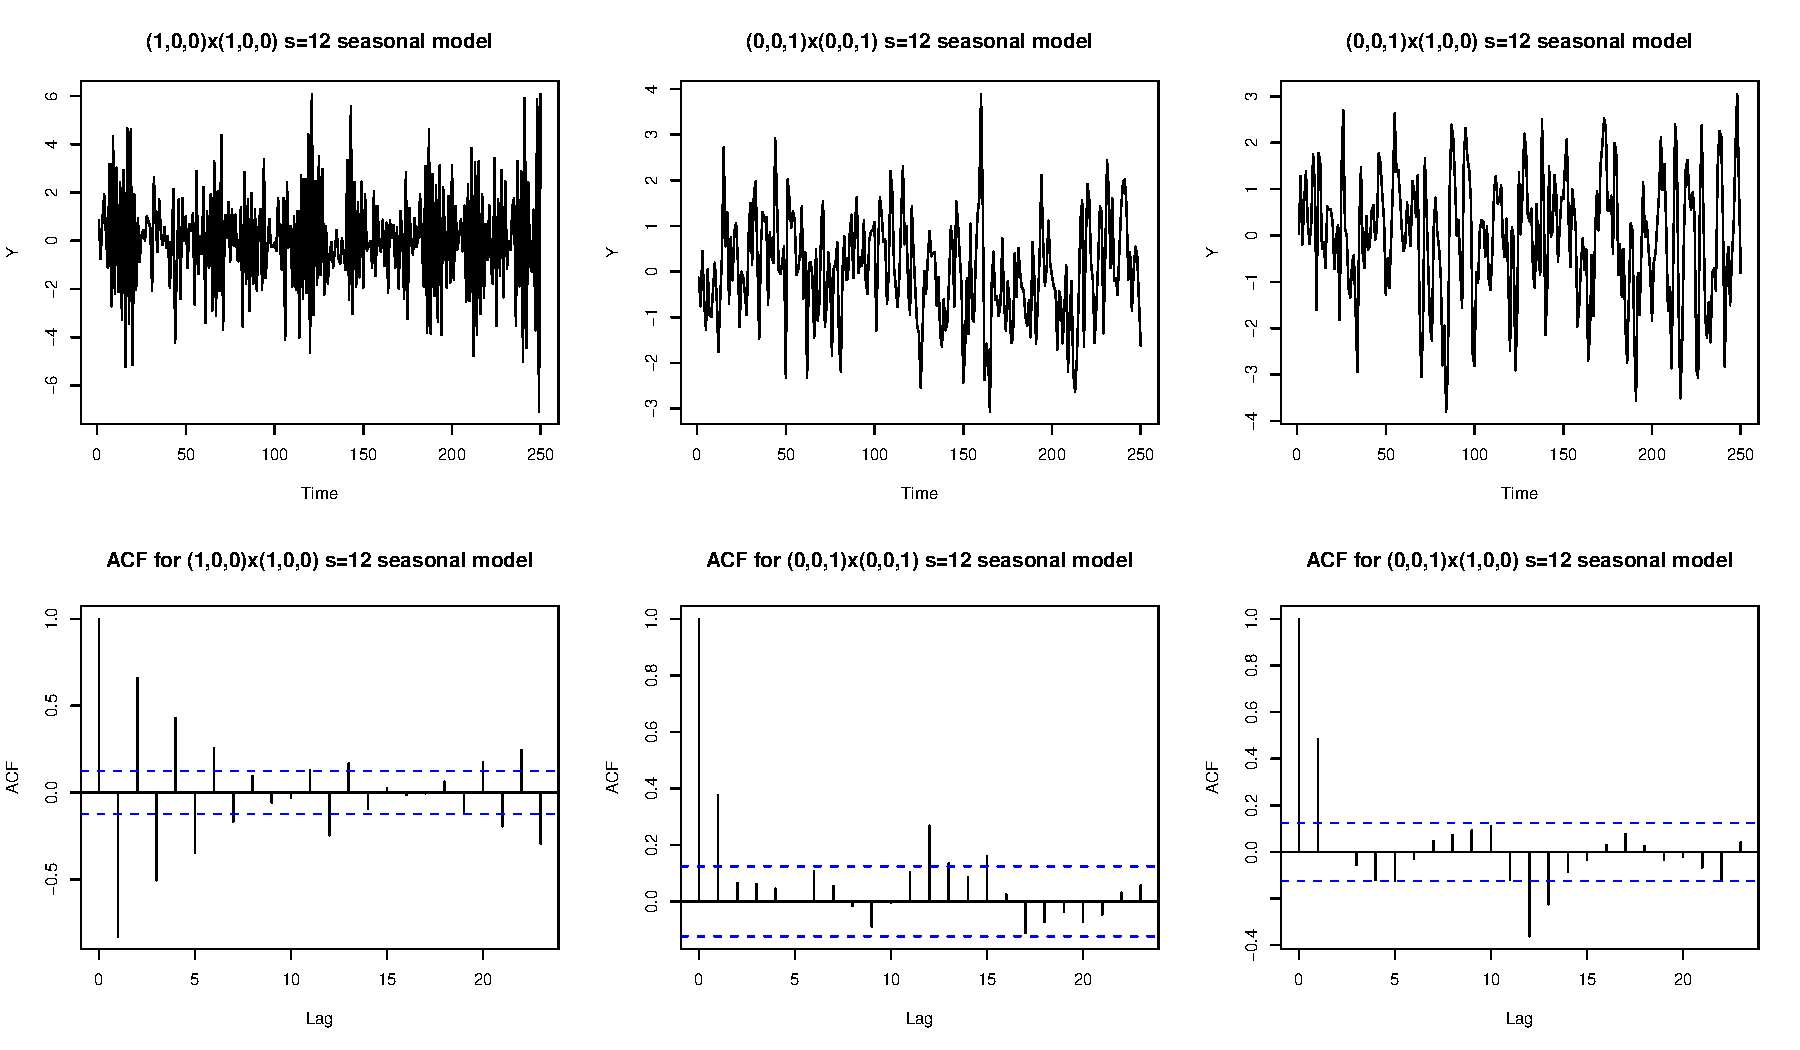
\includegraphics[width=140mm]{seasonalmodels-2.pdf}
    \caption{\textit{Simulation of the last 3 seasonal models in part 4.}}
    \label{fig:p4-2}
\end{figure}

\pagebreak
\section*{Appendices}
All R code used for this assignment is included here. All source code incl. latex code for this report can be found at {\small\url{https://github.com/alphabits/dtu-fall-2011/tree/master/02417/assignment-2}}
\subsection*{(part1.R)}
\lstinputlisting{part1.R}
\subsection*{(ex2.R)}
\lstinputlisting{ex2.R}
\pagebreak
\subsection*{(part2.R)}
\lstinputlisting{part2.R}
\subsection*{(part3.R)}
\lstinputlisting{part3.R}
\subsection*{(part4.R)}
\lstinputlisting{part4.R}


\pagebreak

\begin{thebibliography}{9}

\bibitem{hm}
  Henrik Madsen,
  \emph{Time Series Analysis}.
  Chapman \& Hall/CRC,
  1st Edition,
  2008.

%\bibitem{taleb}
%  Nassim Nicholas Taleb,
%  \emph{The Black Swan}.
%  Random House Trade Paperbacks
%  2nd Edition,
%  2010.

\end{thebibliography}


\end{document}
